Bon, avant toute chose il est important de rappeler\footnote{Comme je
  l'avais déjà dit page~\pageref{sec:phonetics}.} que je ne suis pas
un linguiste professionnel. À vrai dire, avant d'écrire ce livre on
peut dire que je n'avais absolument aucune connaissance du sujet. Mais
il se trouve que mon goût pour apprendre les langues étrangères m'a
amené à approfondir la question. Et comme je n'ai pas envie de dire de
bêtises je vais laisser la parole aux professionnels en me contentant
de les citer, de les paraphraser et de vous transmettre ce que j'en ai
compris. Par conséquent, celles et ceux qui voudraient aller plus loin
sont vivement encouragés à le faire en se procurant les ouvrages cités
qui sont très riches en informations. Pour les autres, il y a deux
possibilités :
\begin{enumerate}
\item Vous n'avez pas envie d'apprendre de nouvelles choses théoriques
  et vous souhaitez directement passer à la pratique. Pas de problème
  ! Dans ce cas il vous suffit d'aller directement à la partie
  suivante page~\pageref{part:vow} pour les voyelles et
  page~\pageref{part:conson} pour les consonnes.
\item Si comme moi vous aimez comprendre les choses sans forcément
  devenir un expert du domaine. Dans ce cas bienvenue dans cette
  partie où j'essaierai de vous communiquer la joie de la découverte
  et ma nouvelle passion pour ce domaine si riche et prometteur.  
\end{enumerate}

\chapter{Pourquoi la phonétique ?}\label{chap:phonetic}

\href{https://fr.wikipedia.org/wiki/Simon_Sinek}{Simon Sinek} qui est
un très bon motivateur explique très bien dans son livre
\href{https://amzn.to/2qY8uMD}{\exEN{Start with why}} que 
le <<~Pourquoi ?~>> est la question fondamentale qu'il faut se poser
en premier. \exEN{Why Phonetics?} est précisément le premier chapitre
du livre \lodge.


\begin{center}
\begin{mdframed}[style=citestyle, frametitle={Extrait du livre \lodge}]
  \exEN{``The reasons for the study of phonetics should be made clear
      at the outset. This chapter is intended to set out the
      reasons why linguists (and any other people interested in
      spoken language of any kind) need phonetics as a tool of
      investigation.''}
\end{mdframed}
\end{center}
  

Ce qui donne en français :

\begin{center}
\begin{mdframed}[style=tradstyle, frametitle={\exFR{Traduction} d'un extrait du livre \lodge}]
  \exFR{<<~Les raisons de l'étude de la phonétique devraient être
    précisées dès le départ. Ce chapitre vise à exposer les raisons
    pour lesquelles les linguistes (et toute autre personne intéressée
    par la langue parlée, quelle qu'elle soit) ont besoin de la
    phonétique comme outil d'investigation.~>>} 
\end{mdframed}  
\end{center}

Le ton est donné ! La phonétique est un outil nécessaire. Nous allons
explorer les explications que notre ami Lodge propose. Et je vous
recommande déjà vivement l'acquisition de son ouvrage.

\newpage
\minitoc
\newpage

\section{Comment décrivons-nous la parole ?}

Le titre de cette section est la traduction du titre de section de son
livre. Il est à noter que l'anglais n'a pas mot véritablement
équivalent au mot parole.

En effet, le titre original utilisait le mot \exEN{speech} qui sert
aussi à traduire le mot discours. En français aussi le mot discours
peut servir aussi bien pour l'écrit que pour l'oral.

Néanmoins le mot parole est plus précis commme nous le reverrons un
peu plus tard.

Revenons à notre section dont je vous propose un premier extrait ci-dessous pour commencer :

\begin{center}
\begin{mdframed}[style=citestyle, frametitle={Extrait du livre \lodge}]
  \exEN{''Traditional education largely ignores spoken language; even
    in drama and foreign language learning, little attention is paid
    to the details of speech in an objective way. We, therefore, need
    a method of describing speech in objective, verifiable terms, as
    opposed to the lay approaches which typically describe sounds as
    'hard', 'soft', 'sharp' and so on, which can only be properly
    understood by the person using such descriptions. Such an approach
    to any subject of study is totally subjective: since only the
    person carrying out the descriptions can understand them, other
    people are expected to be 'on the same wavelength' and clever
    enough to follow them. So, if we are to observe and describe
    speech in any meaningful way, we need some kind of objectively
    verifiable way of doing so. In fact, there are three ways of
    approaching the task.''}
\end{mdframed}  
\end{center}


La première partie de la première phrase est déjà éloquente avant même
que je vous livre la traduction vous avez déjà compris de quoi il
s'agit\dots{} l'oralité est ignorée, niée alors même qu'elle est le
fondement même du langage !

Observons désormais une traduction complète de cet extrait :

\begin{center}
\begin{mdframed}[style=tradstyle, frametitle={\exFR{Traduction} d'un extrait du livre \lodge}]
    \exFR{L'éducation traditionnelle ignore en grande
    partie la langue parlée; même dans l'art dramatique et
    l'apprentissage des langues étrangères, peu d'attention est
    accordée aux détails de la parole d'une manière objective. Nous
    avons donc besoin d'une méthode de description de la parole en
    termes objectifs et vérifiables, opposés aux approches profanes qui
    décrivent généralement les sons comme ``durs'', ``doux'', ``forts'' et
    ainsi de suite, qui ne peut être correctement compris que par la
    personne utilisant de telles descriptions. Une telle approche pour
    n'importe quel sujet d'étude est totalement subjective : puisque
    seul la personne qui exécute les descriptions peut les comprendre,
    les autres sont censés être sur la même longueur d'onde et
    assez intelligents pour les suivre. Donc, si nous devons observer
    et décrire la parole de quelque manière significative, nous avons
    besoin d'un type de manière objectivement vérifiable de le
    faire. En fait, il y a trois façons d'approcher la tâche.} 
\end{mdframed}  
\end{center}


Que ceux qui trouvent que les mots sont un peu trop pompeux ou les
formules trop alambiquées se rassurent. Ce que notre ami Lodge nous
dit ici c'est tout simplement :
\begin{enumerate}
\item Que l'oralité a majoritairement toujours été considéré comme
  inférieure à l'écrit. Et c'est toujours le cas malheureusement. Il
  faut savoir que l'écriture est véritablement répandue que depuis
  l'invention de l'imprimerie. Et il faut attendre le 19ème siècle
  pour que le <<~peuple~>> accède à l'école et donc à la lecture et
  l'écriture. Par conséquent, l'oralité est ultra prépomdérante dans
  l'histoire de l'humanité y compris dans les pays où certains
  essaient d'imposer la supériorité de l'écrit. J'ajouterais que
  l'oralité est une prédisposition biologique ce qui n'est pas le cas
  de l'écrit. Et comme le dit très bien notre ami \href{https://youtu.be/1wsYbQxppRc}{Michel Serres}\footnote{\url{https://youtu.be/1wsYbQxppRc}},
  l'invention de l'écriture est une réduction de la mémoire ou plutôt
  une délégation de mémoire. Que ça soit la Bible ou les récits
  mythologiques Grecs\footnote{Ou d'ailleurs.}, la plupart des textes
  dits <<~sacrés~>> ont d'abord été des mémorisations
  orales\footnote{Ils n'avaient ni la télévision ni les réseaux
    sociaux du coup ils utilisaient davantages leurs réseaux
    neuronaux.}.
\item Que si l'on veut étudier le discours oral on a besoin d'outils
  objectifs. En effet, on ne peut pas se contenter d'expressions
  vagues comme les adjectifs cités dans son extrait. Qu'est-ce qu'un
  \son <<~dur~>> ? Dur à dire si j'ose le petit jeu de mot. Bien sûr
  c'est pratique lorsqu'on veut faire de l'art qui part essence est
  subjectif mais si l'on veut étudier scientifiquement la chose\dots{}
  et bien on a besoin d'une terminologie précise. En clair, notre ami
  Lodge nous dit que l'étude du discours oral doit être traitée comme
  toutes les autres sciences et pour ce faire il lui faut en quelques
  sorte une mathématisation ou si vous préférez une modélisation à
  l'aide de symboles précis.
\end{enumerate}

Voyons à présent quelles sont les trois façons qu'il décrit pour
s'atteler à cette tâche.

\newpage

\section{Première branche de la phonétique}\label{sec:phon-t1}

Commençons par la première branche de la phonétique.

\begin{center}
\begin{mdframed}[style=citestyle, frametitle={Extrait du livre \lodge}]
    \exEN{``What is speech exactly? The expression 'a lot of hot air' is
    rather a good starting point. Speech is made by modulating air in
    various ways inside our bodies. The organs of speech -- the lungs,
    throat, tongue, nose, lips and so on, which we shall discuss in
    detail in Chapter Two -- can be moved into many different
    configurations to produce the different sounds we perceive when
    listening to spoken language. A study of the ways in which these
    \textbf{articulators} of speech behave is called
    \textbf{articulatory phonetics}. In this book the detailed
    investigation of articulation will take up in eight out of the
    nine chapters.''}
\end{mdframed}  
\end{center}


Ce qui donne en français :

\begin{center}
\begin{mdframed}[style=tradstyle, frametitle={\exFR{Traduction} d'un extrait du livre \lodge}]
  \exFR{Qu'est-ce que la parole ? L'expression ``beaucoup
    d'air chaud'' est plutôt un bon point de départ. La parole est
    faite en modulant l'air de diverses façons à l'intérieur de notre
    corps. Les organes de la parole -- les poumons, la gorge, la langue,
    le nez, les lèvres etc\dots{}, dont nous allons discuter
    en détail dans le chapitre deux -- peuvent être déplacés dans de
    nombreuses configurations différentes pour produire les différents
    sons que nous percevons quand nous écoutons la langue parlée. Une étude
    des façons dont ces \textbf{articulateurs} du discours se
    comportent est appelée \textbf{phonétique articulatoire}. Dans ce
    livre, l'enquête détaillée sur l'articulation occupera huit des
    neuf chapitres.}
\end{mdframed}  
\end{center}

De la même façon que notre ami Lodge l'a fait dans son livre, ici
aussi nous nous occuperons principalement de la phonétique
articulatoire. En bref, cela signifie que l'on va se focaliser sur la
façon de produire les sons. D'ailleurs, même si j'ai donné tous les
noms techniques, il n'est nullement question de théorie pour pratiquer
la phonétique et amélioration de sa prononciation, tout est question
d'écoute et de répétition. Mais comme l'a très justement souligné
notre ami Lodge, l'utilisation d'une terminologie précise a pour but
et avantage de nous permettre de nous y retrouver et de voir les
différences entre les sons.

Juste pour la culture poursuivons la description de notre ami Lodge. 

\newpage

\section{Deuxième branche de la phonétique}\label{sec:phon-t2}

Passons à la deuxième branche de la phonétique.

\begin{center}
\begin{mdframed}[style=citestyle, frametitle={Extrait du livre \lodge}]
  \exEN{``Basically, air is pushed out of the body and disturbs the outside
  air between the speaker and anyone in the vicinity who can hear
  him/her. These disturbances are known as \textbf{pressure
    fluctuations}, which in turn cause the hearer's eardrum to
  move. The molecules of the air move together and then apart in
  various ways, producing a \textbf{sound wave}. The study of the
  physical nature of sound waves is \textbf{acoustic
    phonetics}. We shall look at this aspect of speech and the
  relationship of articulation to acoustic effects in Chapter Nine.''}
\end{mdframed}  
\end{center}

    
Ce qui donne en français :

\begin{center}
\begin{mdframed}[style=tradstyle, frametitle={\exFR{Traduction} d'un extrait du livre \lodge}]
  \exFR{Fondamentalement, l'air est expulsé du corps et perturbe
    l'air extérieur entre l'orateur et toute personne dans le
    voisinage qui peut l'entendre. Ces perturbations sont
    appelées \textbf{fluctuations de pression}, qui à leur tour
    provoquent le mouvement du tympan de l'auditeur. Les molécules de
    l'air se déplacent ensemble puis se séparent de diverses manières,
    en produisant une \textbf{onde sonore}. L'étude de la nature
    physique des ondes sonores est l'\textbf{acoustique
      phonétique}. Nous allons regarder cet aspect du discours et la 
    relation d'articulation aux effets acoustiques dans le chapitre neuf.}
\end{mdframed}  
\end{center}


Ceci est très intéressant et nous conduirait à une analyse physique du
\son qui serait également valable pour la musique. D'ailleurs, en
général, lorsqu'on parle d'acoustique la première chose qui vient à
l'esprit c'est la musique\footnote{À moins que je ne sois le seul à
  penser comme ça.}. Néanmoins, pour ce premier livre je me suis
restreint à la phonétique articulatoire. Et puis je vais vous faire
une petite confidence cette partie sur la linguistique est celle que
j'ai écrit en dernier parce que je me suis dit que faire une
introduction à la phonétique sans même la définir
sérieusement\footnote{Ben oui la petite définition Wikipédia c'est
  bien gentil mais c'est un peu léger.} ça serait un peu abuser. Du
coup ça m'a mis l'eau à la bouche pour un livre plus conséquent sur le
sujet. Mais pour l'instant mon approche est purement pragmatique,
comme utiliser ces outils pour améliorer et accélérer l'acquisition
d'une langue (ici l'anglais).

\newpage

\section{Troisième branche de la phonétique}\label{sec:phon-t3}

Observons maintenant la dernière branche de la phonétique.

\begin{center}
\begin{mdframed}[style=citestyle, frametitle={Extrait du livre \lodge}]
  \exEN{``The third way of considering speech, \textbf{auditory
      phonetics}, deals with the ways in which speech affects and is
    interpreted by the hearer(s). This aspect of the investigation of
    speech will not be considered in this book.''}
\end{mdframed}  
\end{center}

Ce qui donne en français :

\begin{center}
\begin{mdframed}[style=tradstyle, frametitle={\exFR{Traduction} d'un extrait du livre \lodge}]
  \exFR{La troisième façon de considérer la parole, la
    \textbf{phonétique auditive}, traite des façons dont la
    parole affecte et est interprété par le ou les auditeur(s). Cet
    aspect de l'étude de la parole ne sera pas considéré dans ce livre.}
\end{mdframed}  
\end{center}


Maintenant je pense que vous avez un aperçu assez intéressant de ce
qu'est la phonétique. En particulier, même si nous nous restreindrons
à la phonétique articulatoire, il me semblait important de montrer la
rigueur scientifique qu'il y a derrière cette discipline qui ne se
résume pas aux pauvres petites transcriptions que l'on voit dans les
dictionnaires et dont les professeurs de langues ne nous ont jamais
parlé ni au collège ni au lycée.

Bien entendu notre cher ami Lodge ne s'adresse pas au
débutant\footnote{Encore qu'avec un peu de patience et de persévérance
tout le monde peut lire et comprendre son livre.}, je pense que sa
description est assez claire.

Nous en avons fini avec la description de la théorie phonétique. Avant
de rentrer dans le vif du sujet je vais tout de même faire un autre
petit chapitre similaire. Pourquoi ? Parce que l'autre source que j'ai
sélectionné est un manuel à l'usage de locuteurs non anglophones donc
son approche pourra nous être utile. Et de plus cette fois on brosse
un portrait général de la linguistique.

\newpage
\minitoc
\newpage

\chapter{La linguistique ça vous parle ?}\label{chap:linguistic}

La phonétique, normalement maintenant, vous savez à peu près ce que
c'est. Mais qu'en est-il de la linguistique ?

Ben il se retrouve que la phonétique en est une de ses branches.

\begin{center}
    \begin{figure}[h]
      \centering
        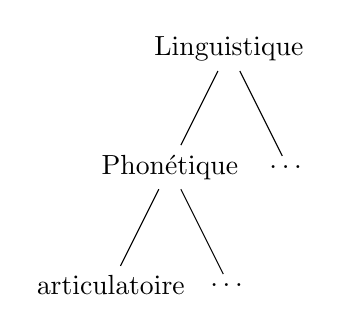
\begin{tikzpicture}
          \node {Linguistique}
          child { node {Phonétique}  
            child { node { articulatoire } }
            child { node { \dots } }
          }
          child { node {\dots} } 
          ;
        \end{tikzpicture}
    \caption{Branches de la linguistique}
    \label{fig:branch-phon}
  \end{figure}
\end{center}
Cela vous paraît peut être surprenant que je m'amuse à remonter les
branches. Pourtant c'est une démarche assez naturelle. On a
fondamentalement deux façons d'étudier un domaine.

\begin{enumerate}
\item La première consiste à partir du général  pour aller vers le
  particulier.
\item La seconde consiste à faire l'inverse.  
\end{enumerate}

 L'objet de ce livre étant de traiter de la phonétique anglaise il m'a
 paru plus opportun de démarrer avec une vue d'ensemble de la
 phonétique. Mais il me semble tout de même nécessaire de dessiner le
 contour de ce qu'est la linguistique qui, hélas, n'est pas une
 science très connue du grand public alors qu'elle est probablement la
 plus fondamentale.

 Au commencement était le verbe\footnote{Il est amusant de voir qu'en
   anglais ce n'est pas tout à fait pareil \exEN{In the beginning was
     the Word} qui se traduit littéralement par \exFR{Au commencement
     il y avait le Mot}.} aurait dit l'autre, et ce n'est pas pour
 rien, le langage oral est ce que nous partageons tous nous autres
 êtres humains. Quelle que soit votre activité, dans tous les cas vous
 communiquez par le langage.

 \'Etrangement à l'école nous ne l'étudions pas beaucoup ce
 langage. Lors des petites classes on nous fait apprendre les règles
 par c{\oe}ur puis on passe vite à la littérature (dès le collège) ou
 à la philosophie (au lycée). Il en va de même pour les langues
 étrangères. Pourtant lorsqu'on y réfléchi c'est tout de même étrange
 de se dire que nous partageons tous la même faculté de produire du
 langage mais que l'endroit où nous naissons va considérablement
 affecter les règles que nous allons utiliser pour le produire.

 Bref, sans plus attendre, laissons la parole aux professionnels que sont
 messieurs \textsc{Paul Burleigh} et \textsc{Peter Skandera} avec leur
 livre \href{https://amzn.to/2HV8BzG}{A Manual of English Phonetics and
  Phonology} qui était à la base destiné à un public de langue allemande.

\newpage
\minitoc
\newpage

\section{Prescriptivisme et descriptivisme}

Le débat entre prescriptivistes et descriptivistes est un éternel
débat dont j'avais déjà parlé dans cet
\href{http://doyouspeakenglish.fr/prescriptiviste-ou-descriptiviste/}{article}
de
blog\footnote{\url{http://doyouspeakenglish.fr/prescriptiviste-ou-descriptiviste/}}. Malheureusement
en France nous n'avons pas vraiment le droit de nous exprimer
puisqu'il existe une institution qui décide pour tout le monde des
règles de la langue française. Du coup, cela pourra paraître, au
premier abord, être une querelle de spécialiste. Mais il n'en est
rien, et ce serait une erreur de prendre ça à la légère ! C'est une
véritable question de fond !

\begin{center}
\begin{mdframed}[style=citestyle, frametitle={Extrait du livre \bs}]
  \exEN{``From ancient times until the present, language purists have
    believed that the task of the grammarian is to \emph{prescribe}
    (rather than \emph{describe}) correct usage that all educated
    people should use in speaking and
    writing. \textbf{Prescriptive} language scholars have
    laid down rules that are often based on Latin and Greek, on a
    classical canon of literary works, on the origin of particular
    words, on logic, or simply on their personal likes and
    dislikes. Prescriptivists have been criticised for not taking
    sufficient account of ongoing language change and stylistic
    variation. By contrast, the aim of linguistics is to
    \emph{describe} language objectively and
    systematically. \textbf{Descriptive} linguists observe
    and analyse language as it is used naturally in any given speech
    community [\emph{\textgerman{Sprachgemeinschaft}}], and they
    attempt to discover the rules and regularities of the underlying
    language system, or code.''}
\end{mdframed}  
\end{center}

Dès la première ligne on observe à quel point la question est
ancienne. Il est amusant de remarquer que le mot prescriptiviste a la
même racine que le verbe prescrire qui est utilisé par le médecin
lorsque nous sommes malades. Cela voudrait-il dire que certaines
personnes penseraient que d'autres sont malades de la langue ?

Occupons-nous désormais de la traduction.

\begin{center}
\begin{mdframed}[style=tradstyle, frametitle={\exFR{Traduction} d'un extrait du livre \bs}]
  \exFR{Depuis les temps anciens jusqu'à nos jours, les puristes de la
    langue croyaient que la tâche du grammairien est de \emph{prescrire}
(plutôt que \emph{décrire}) l'usage correct que tous les gens éduqués
devraient utiliser pour parler et écrire. Les professeurs de langues
\textbf{prescriptifs} ont établi des règles qui sont souvent
basées sur le latin et le grec, sur des canons classiques d'{\oe}uvres
littéraires, sur l'origine de certains mots, sur la logique, ou simplement sur
leurs goûts personnels en fonction de ce qu'ils aiment et n'aiment
pas. Les prescriptivistes ont été critiqués pour ne pas tenir compte
suffisamment du changement de la langue en usage et des variations
stylistiques. En revanche, le but de la linguistique est de
\emph{décrire} le langage objectivement et systématiquement. Les
linguistes \textbf{descriptivistes} observent et analysent
le langage tel qu'il est utilisé naturellement dans n'importe quel
discours donné dans une communauté
[\textgerman{\emph{Sprachgemeinschaft}}], et ils tentent de découvrir
les  règles et les régularités du système de langue sous-jacent, ou
code.}
\end{mdframed}  
\end{center}


Pour la faire simple on va dire que les prescriptivistes sont les
conservateurs et les descriptivistes les progressistes. Alors vu de
France c'est un peu compliqué parce que nous sommes fondamentalement
dans un pays prescriptiviste puisque une vieille bande d'illuminés
qui se prétendent immortels ont un droit absolu sur la façon de dicter
les lois de la langue française.

Bien heureusement, en France comme dans tous les pays, ce sont les
locuteurs qui font la langue et non les législateurs. Néanmoins ces
derniers ont tout de même un pouvoir fort sur la façon dont les
esprits sont éduqués. Et il est bien difficile de sortir du
conditionnement dont on a été victime durant son éducation il faut
bien le reconnaître.

Les linguistes étant par définition ceux qui observent et décrivent la
langue il serait intéressant d'en entendre parler avant de passer le
bac. Cela me semble plus concret et utile que de savoir que
Jean-Jacques\footnote{Ce même Jean-Jacques qui a écrit des choses
  beaucoup plus intéressantes comme le \href{https://www.rousseauonline.ch/pdf/rousseauonline-0004.pdf}{contrat social} par exemple.} s'est pris une fessée et l'a raconté dans son autobiographie\dots{}

\newpage
\section{Parole vs. langue et performance vs. compétence}

\begin{center}
\begin{mdframed}[style=citestyle, frametitle={Extrait du livre \bs}]
  \exEN{``In order to separate the two meanings of the word
    \emph{language} illustrated in the last sentence of the previous
    paragraph, the Swiss linguist Ferdinand de Saussure (1857-1913)
    proposed the French terms \textbf{parole} to refer to
    actual language use (i.e. to concrete utterances) and
    \textbf{langue} for a speech community's shared
    knowledge of a language (i.e. for the language system).''}  
\end{mdframed}  
\end{center}


Ce qui donne en français :

\begin{center}
\begin{mdframed}[style=tradstyle, frametitle={\exFR{Traduction} d'un extrait du livre \bs}]
  \exFR{Afin de séparer les deux significations du mot \emph{langage}
    illustré dans la dernière phrase du précédent paragraphe, le
    linguiste suisse Ferdinand de Saussure (1857-1913) proposa les
    termes français \textbf{parole} pour se référer à l'utilisation réelle
    de la langue (c'est-à-dire aux énoncés concrets) et
    \textbf{langue} pour un discours communautaire qui partage la
    connaissance d'une langue (c'est-à-dire pour le système
    linguistique).} 
\end{mdframed}  
\end{center}


On voit sur cet extrait que le français offre plus de précision grâce
aux mots parole, langue et langage là où l'anglais utilise
\exEN{speech} à la fois pour le discours écrit et oral ainsi que
\exEN{language} à la fois pour langue et langage. Il est important de
signaler également qu'à l'époque de Saussure, et ce jusqu'à la seconde
guerre mondiale, le français était la \exLT{lingua franca}, la langue
dominante, la langue noble. Rôle joué par l'anglais désormais. 

\begin{center}
\begin{mdframed}[style=citestyle, frametitle={Extrait du livre \bs}]
  \exEN{``A similar dichotomy was put forward by the American linguist
    Noam Chomsky (b. 1928), who used the terms \textbf{performance}
    and \textbf{competence} to refer to largely the same
    concepts. Chomsky, however, put more emphasis on the individual
    nature of language. Performance, then, is the actual language use
    of an individual speaker, and competence is that individual
    speaker's knowledge of the language. Chomsky later replaced these
    terms with \textbf{E(xternalised)-language} and
    \textbf{I(nternalised)-language}, but the new terms are rarely used.''}  
\end{mdframed}  
\end{center}

Ce qui donne en français :

\begin{center}
\begin{mdframed}[style=tradstyle, frametitle={\exFR{Traduction} d'un extrait du livre \bs}]
  \exFR{Une dichotomie similaire a été mise en avant par le linguiste
    américain Noam Chomsky (né en 1928), qui utilisait les termes
    \textbf{performance} et \textbf{compétence} pour se référer
    largement aux mêmes concepts. Chomsky, cependant, met plus l'accent
    sur la nature individuelle de la langue. La performance, alors, est
    l'utilisation réelle de la langue d'un locuteur individuel, et la
    compétence est la connaissance personnelle du locuteur de la
    langue. Chomsky a plus tard remplacé ces termes avec \textbf{langue
      (E)xternalisée} et \textbf{langue I(nternalisée)}, mais les
    nouveaux termes sont rarement utilisés.}   
\end{mdframed}  
\end{center}


Là on commence à s'aventurer sur un domaine plus technique donc je
n'irais pas plus loin dans la profondeur. J'ai cité ce passage car
Noam Chomsky est le scientifique qui a le plus contribué dans le
domaine de la linguistique. Par conséquent il était très important de
citer au moins un de ses apports. La section suivante sera plus
intéressante du point de vue de la vulgarisation.

\newpage

\section{Les quatre domaines de base de la linguistique}

Voyons à présent les quatre branches majeures de la linguistique de
base, telle qu'elle a été conçue à son origine.

\begin{center}
\begin{mdframed}[style=citestyle, frametitle={Extrait du livre \bs}]
  \exEN{``The system or structure of a language (langue or competence)
    can be described at four different levels, which form the core
    areas of linguistics, sometimes called \emph{microlinguistics}:
    (1) \textbf{Phonetics} and \textbf{phonology} deal with
    pronunciation, or, more precisely, with speech sounds and the
    sound system. (2) \textbf{Morphology} covers the structure of
    words. (3) \textbf{Syntax} explains sentence patterns. (Morphology
    and syntax, often combined into \emph{morphosyntax}, have
    traditionally been referred to as \emph{grammar}.) (4)
    \textbf{Lexicology} and \textbf{semantics} describe the
    vocabulary, or lexicon, and explore different aspects of meaning.''}  
\end{mdframed}  
\end{center}

Derrière ces noms qui peuvent éventuellement faire peur se cache des
opérations\footnote{En ce sens la linguistique est véritablement très
  proche des mathématiques, d'ailleurs en informatique théorique
  l'arithmétique est considérée comme un langage avec un alphabet à 10
symboles si on utilise le système décimal par exemple.} que l'on fait
instinctivement.

Par exemple pour la phonétique et la phonologie du français nous
n'avons pas eu besoin de les théoriser car nous les avons appris
empiriquement par écoute et imitation des sons.

Il en va de même pour la formulation des mots (morphologie); d'ailleurs je suis sûr
qu'il vous est déjà arrivé d'inventer des mots avant même de savoir
lire ou écrire.

Pour ce qui est de la syntaxe c'est un peu plus délicat mais pour ce
qui est des phrases de base elles se construisent également
instinctivement. C'est précisément sur la syntaxe que les esprits
chagrins revendiquent le prescriptivisme.


Passons maintenant à la traduction :

\begin{center}
\begin{mdframed}[style=tradstyle, frametitle={\exFR{Traduction} d'un extrait du livre \bs}]
  \exFR{Le système ou la structure d'une langue (langue ou compétence)
    peut être décrit à quatre niveaux différents, qui forment le
    c{\oe}ur des domaines de la linguistique, parfois appelé
    \emph{microlinguistique}: (1) La \textbf{phonétique} et la
    \textbf{phonologie} traitent de la prononciation, ou, plus
    précisément, des sons de la parole et du système auditif. (2)
    La \textbf{morphologie} couvre la structure des mots. (3) La
    \textbf{syntaxe} explique les modèles de phrases. (Morphologie et
    syntaxe, souvent combinées en \emph{morphosyntaxe}, ont
    traditionnellement été dénommé \emph{grammaire}.) (4) La
    \textbf{lexicologie} et la \textbf{sémantique} décrivent le
    vocabulaire, ou lexique, et explorent différents aspects de la
    signification.}    
\end{mdframed}  
\end{center}


À présent nous avons une vue d'ensemble qui me semble assez
claire.

Finalement, selon moi, la linguistique traite véritablement de
la façon dont nous communiquons.

En partant de la façon dont nous produisons et recevons les sons
(c'est précisément le rôle de la phonétique et de la phonologie).

Puis elle analyse la façon dont nous construisons les mots (la
morphologie) et les phrases (la syntaxe) par ajacement de ces
derniers.

Enfin, nos communications ont un sens (la sémantique).

Il est véritablement curieux que la linguistique ne soit pas enseignée
dès le plus jeune âge car c'est véritablement l'outil le plus
important que tout être humain devrait maîtriser ou du moins connaître les bases.

J'arrête ici avec les citations mais je vous dresse tout de même
brièvement la liste des autres branches de la linguistique (qu'on
appelle la \emph{macrolinguistique} afin d'aiguiser votre curiosité
car vous allez voir cela touche à de nombreux domaines. Notamment des
domaines qui concernent les nouvelles technologies.

\begin{enumerate}
\item La \textbf{dialectologie} qui est l'intersection entre la
  linguistique et la géographie. Par exemple en anglais cela
  consisterait à se pencher sur les variations entre les différentes
  variations selon que l'on est en Angleterre, en \'Ecosse, au
  Canada\dots{} ou ailleurs.
\item La \textbf{socio-linguistique} qui comme son nom l'indique mêle
  sociologie et linguistique. Si l'on reprend l'exemple de l'anglais
  on pourrait par exemple étudier le fait que l'accent RP était une
  façon de montrer son appartenance à une classe sociale élevée.
\item L'\textbf{ethno-linguistique} qui est à la frontière entre
  l'anthropologie, l'ethnologie et la linguistique. On peut voir que les
  trois premiers domaines sont assez proches.
\item L'\textbf{analyse du discours}, la \textbf{linguistique
    textuelle} et \textbf{stylistique} s'occuppent cette fois des
  variations au niveau supérieur que les phrases. Pour l'oral par
  exemple cela va consister à analyser des conversations, des
  discours, des conférences et ainsi de suite. Concernant l'écrit, on
  étudiera les lettres personnelles, les articles de presse, ou encore
  les papiers universitaires.
\item La \textbf{linguistique comparative} décrit les similarités et
  différences entre des langues modernes. Par exemple entre l'anglais
  et le français.
\item La \textbf{psycholinguistique} à cheval entre la psychologie et
  la linguistique. Elle s'intéresse notamment à l'apprentissage.
\item La \textbf{neurolinguistique} qui s'occupe des connexions entre
  le langage et le système nerveux.
\item La \textbf{linguistique computationnelle} qui est probablement
  la plus récente et qui connaît un essor considérable grâce à
  l'avènement des nouvelles technologies et en particulier
  l'intelligence artificielle. C'est dans cette branche de la
  linguistique que l'on s'occupe du traitement automatique des langues
  comme par exemple les outils de traduction automatique en ligne ou
  sur application mobile ou encore les outils de reconnaissance
  vocale.   
\end{enumerate}

Comme vous avez dû vous en rendre compte la linguistique couvre
potentiellement l'ensemble du spectre des connaissances humaines. Je
vous avouerais que je suis particulièrement sensible à la dernière
branche citée. J'espère vous avoir communiqué mon appétit pour la
découverte de ce champ d'investigation aussi vaste qu'intéressant et
je vous invite désormais à vous concentrer sur la
phonétique\footnote{À partir de maintenant je ne parlerai que de la
  phonétique articulatoire parce que c'est celle que l'on trouve dans
  les dictionnaires et que nous pratiquons lorsque nous produisons les
  sons.}, et en particulier celle de l'anglais.

\begin{center}
  \begin{figure}[h]
    \centering
    \includegraphics[scale=.65]{../img/burleigh-skandera/app-phon-bs}
    \caption{Organes de la parole, issu du livre \bs}
    \label{fig:app-phon}
  \end{figure}
\end{center}

Je vous souhaite une bonne étude à l'aide de ce guide.

\newpage
\minitoc
